\subsection{Mineração}
O segundo passo após coletar os dados é rodar scripts de mineração. Uma das maiores dificuldades é como manipular os dados de maneira incremental. Desde que a pesquisa teve inicio, muitas ideias surgiram, novos pontos de vistas e novos dados a serem minerados. Foi adotado uma propriedade chamada \textit{processing\_version}, essa propriedade marca o documento com a versão do processamento dele.

Dentro da pasta \textit{dumont/tasks/processing} existe duas pastas, uma para processar usuários e outra para processar tweets, ambas exportam vários estágios de processamento, esse estágio é exportado e passado para uma classe chamada \textit{Processor} localizada no arquivo \textit{dumont/tasks/processing/\_\_init\_\_.py}, o nível de processamento base é o 0 (nível inserido na hora que o coletor salva do dado no banco), a partir disso é possível atualizar o processamento por um script (no caso existe a possibilidade de consumo da fila, porem, como já dito essa abordagem esta contida no anexo 1).

Quando o coletor foi configurado, automaticamente todos os dados necessários para o processamento já foram preenchidos. A tarefa de processamento é responsável por:

\begin{itemize}
    \item Remoção de \textit{stop-words}: Existem palavras que prejudicam a analise textual por não serem essenciais ou estarem colocadas de maneira equivocada. Um dos processos retira esse tipo de ruído do texto.
    \item Arvore Léxica: Criar uma arvore léxica baseada na frase original do tweet e na frase que já foi tratada removendo as \textit{stop-words}.
    \item Analise de Sentimento: Utilizando a API do Google Language é retirado o sentimento da frase original e da frase tratada também.
\end{itemize}

Para obter esses dados basta rodar o comando \textit{docker-compose -f docker-compose.dev.yml up tasks}. Com esses dados já é possível ter alguma noção de informações relevantes dos textos, porém ainda é necessário de embasamento técnico, ou seja, um dado especialista que possa orientar a máquina a utilizar as demais propriedades mapeadas para localizar um delta em comum.

Existe um outros serviços contidos dentro do projeto o \textit{dumont/specialist\_api} e \textit{dumont/specialist\_app} que gera uma API e uma interface gráfica para injeção de dados especialistas. Para subir ambos os serviços basta utilizar o comando \textit{docker-compose -f docker-compose.dev.yml up specialist\_app}. Entretanto, é necessário de um usuário para injetar as analises, é possível criar o documento na mão dentro do mongo, porem, existe um binário dentro da pasta chamado \textit{dumont/create\_specialist}, basta executa-lo passando o e-mail e ele te devolvera uma senha aleatória. Então basta acessar \textit{\url{http://127.0.0.1:3000/}} e utilizar os dados para entrar no sistema. Logo que autenticado você encontrara uma tela igual a da figura \ref{fig:specialist}, nela existe o tweet, uma área para adicionar perguntas da EADS relacionadas, e um local onde pode-se identificar palavras chaves dentro daquele tweet.

\begin{figure}
    \centering
    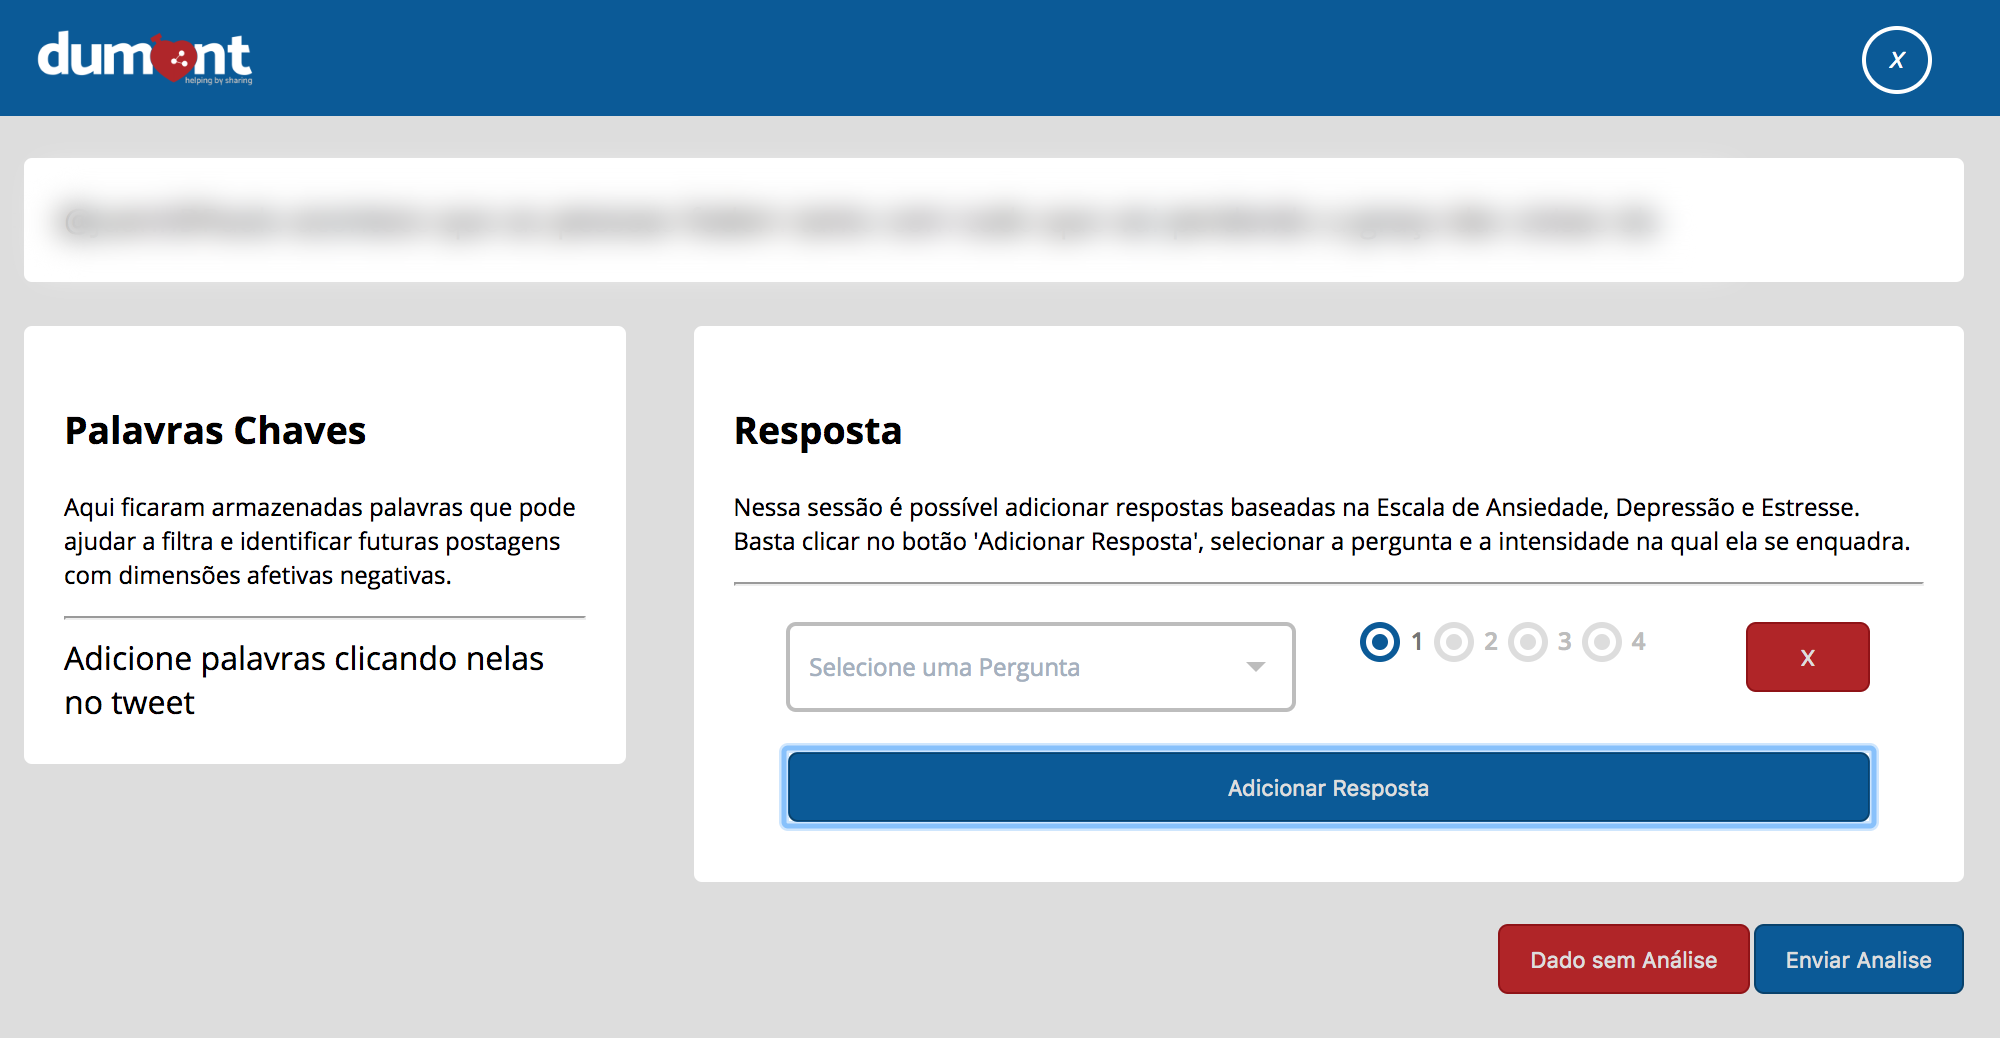
\includegraphics[width=1\textwidth]{imagens/specialist.png}
    \caption{Interface de captação de respostas dos especialistas}
    \label{fig:specialist}
\end{figure}

Com o sistema rodando, e dados sendo coletados e analisados é necessária uma amostragem para melhor assertividade e desenvolvimento. Durante a pesquisa, em uma preliminar foram coletados mais de 160GB de dados. A amostra foi tirada antes mesmo da inserção de dados especialistas, logo é necessário conhecer os \textit{scripts} de seleção do dumont.
